\newpage
\section{Durchführung}
Verwendet wird eine Kupfer-Röntgenröhre mit einem LiF-Kristall und einem
Geiger-Müller-Zähler. Die Beschleunigungsspannung beträgt $35\;$kV mit
einem Emissionstrom von $1\;$mA.

\subsection{Bragg-Bedingung}
Der LiF-Kristall wird auf einen festen Kristallwinkel von $\Theta=14$° 
eingestellt. Mithilfe des Geiger-Müller-Zählers wird in eimen Winkelbereich
von $\alpha_{GM}=[26°,30°]$ mit einer Schrittweite von $0,1$° die Strahlungsrate $N$
gemessen.

\subsection{Emissionsspektrum}
Das Röntgensektrum wird in einem Winkelbereich von $\Theta=[4°,26°]$
mit einer Schrittweite von $0.2$°  gemessen. 
Aus den Daten können nun die charakteristischen Linien 
$K_{\alpha}$ und $K_{\beta}$, der Bremsberg, die minimale
Wellenlänge vgl. \ref{eqn:minW} und die Abschirmkonstenten $\sigma$ bestimmt werden.
Die Halbwertsbreite (Full Width at Half Maximum) der scharfen Linien 
im Spektrum liefern dann mit !ref! eine Aussgabe über das Auflösungsvermögen $A$.
\subsection{Absorbtionsspektrum}
Für verschiedene Absorber (Brom, Zink, Gallium, Rubidium, Zirkonium)
wird ein Absorbtionsspektrum im geeigneten Winkelbereich vermessen.
Mit Hilfe der Absorbtionsenergien kann die Abschirmzahl $\sigma_K$ 
ermittelt werden.
Betrachtet werden dann die Energieübergänge der gemessene K-Kanten. 
\begin{figure}
    \centering
    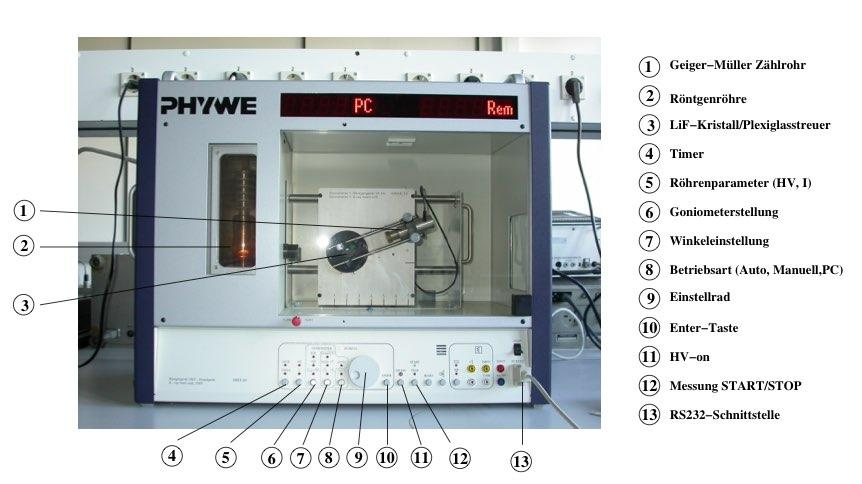
\includegraphics[width=0.8\textwidth]{plots/Apperatur.jpg}
    \caption{Das verwendetete Röntgengerät \cite[4]{anleitung}.}
\end{figure}




\label{sec:Durchfuehrung}
